\documentclass[12pt]{article}
\usepackage[english]{babel}
\usepackage[utf8x]{inputenc}
\usepackage[T1]{fontenc}
\usepackage{listings}
\usepackage{tikz}
\usepackage{/Users/songye03/Desktop/math_tex/style/quiver}
\usepackage{/Users/songye03/Desktop/math_tex/style/scribe}

\begin{document}
Songyu Ye

\today

\hfill

This is my understanding of Delzant's theorem, sympletic reduction, and (maybe) projective GIT quotients.

\section{Hamiltonian vector fields and moment maps}
\subsection{Crash course in complete vector fields}
Recall differential geometry. There is a correspondence \begin{align*}
	\set{\text{actions of $\R$ on $M$}} & \longleftrightarrow \set{\text{complete vector fields on $M$}} \\
	\psi                                & \mapsto X_p = d\psi_t(p)/dt|_{t=0}                             \\
	\exp(tX)                            & \leftarrow X
\end{align*} where we are corresponding the "flow of $X$" with the "vector field generated by $\psi$.
In particular, if I have an action of $\R$ on $M$, then I get an infinitesimal action which at each point of $M$
tells me how to diffrentiate smooth functions, i.e. a tangent vector. On the other hand, if I have a complete vector field,
I can think about its integral curve, which are smooth curves whose velocite at each point is the value
of the vector field. Since the vector field is complete, the integral curves exist for all time
and so I get an action of $\R$ on all of $M$.

\hfill

The correspondence we really care about is the one with the adjective "symplectic" on both sides.

\begin{example}
	$V = x^1\partial/\partial x^1 + \dots + x^n \partial/\partial x^n$ is the "radial" vector field on $\R^n$.
	It is smooth since each of its coordinate functions is smooth. What is $\partial/\partial x^n$?
	Recall that geometric tangent vectors act on smooth functions via the directional derivative.
	By letting them act on the coordinate functions, one sees that they are isomorphic to derivations. Thus
	we just think about tangent vectors as derivations.
\end{example}

\begin{example}
	$\partial/\partial \theta$ on $S^1$. We can only talk about this vector field on a given chart, but
	any other angle coordinate differens from $\theta$ by an additive constant in a neighborhood of a point,
	so there is a globally defined vector field on $S^1$. This says that the circle is parallelizable.
\end{example}

\hfill

The geometric objects associated to vector fields are their integral curves. Consider the case
in which for each $V$ on $M$ there is a unique integral curve for $V$ starting at $p$, existing for all $t\in \R$.

\hfill

Then we say that $V$ is complete.
\begin{example}
	Every compactly supported smooth vector field on a smooth manifold is complete.
	Every left invariant vector field on a Lie group is complete.
\end{example}

\subsection{Hamiltonian vector fields}
Consider $(M,\omega)$ a symplectic manifold and some $f\in C^\infty(M)$.
The Hamiltonian vector field of $f$ is \begin{align*}
	X_f = \omega^\sharp(df)
\end{align*} where $\omega^\sharp:T^*M\to TM$ is the isomorphism induced by $\omega$. This vector field
then satisfies \begin{align*}
	i_{X_f}\omega = df
\end{align*}

\begin{example}
	There is a theorem of Darboux which says that in a neighborhood of any point in $M$ there are
	local coordinates $(x^1,\dots,x^n,y^1,\dots,y^n)$ such that $\omega = \sum dx^i\wedge dy^i$.
	In Darboux coordinates, Hamiltonian vector fields look like \begin{align*}
		X_f = \sum \frac{\partial f}{\partial y^i}\frac{\partial}{\partial x^i} - \frac{\partial f}{\partial x^i}\frac{\partial}{\partial y^i}
	\end{align*}
	On $\R^{2n} = \C^n$, the Darboux coordinates are defined globally and
	they are known as the canonical symplectic form on $\C^n$.
\end{example}

\begin{definition}
	$X$ is symplectic if $\omega$ is invariant under the flow of $X$.
	$X$ is Hamiltonian if there is some $f\in C^\infty(M)$ so that $X = X_f$.
\end{definition}

\begin{proposition}
	$X$ is symplectic if $i_X\omega$ is closed. $X$ is Hamiltonian if $i_X\omega$ is exact.
\end{proposition}
Therefore to say that a sympletic action of $\R$ on $M$ is Hamiltonian
is to say that there is a smooth symplectic vector field $X$ so that $X$ is the
Hamiltonian of some $f\in C^\infty(M)$ and that $X$ corresponds to the infinitesimal
action of $\R$ on $M$.

\subsection{Cartan's magic formula}
We need Cartan's magic formula to do some examples.

\begin{definition}
	$\mf{L}_X$ is the Lie derivative. It is a map \begin{align*}
		\mf{L}_X:\mf{X}(M)\to \mf{X}(M) \\
		\mf{L}_X(Y)(f) = X(Y(f)) - Y(X(f))
	\end{align*}
\end{definition}

The Lie derivative is a map of vector fields which extends to a map of tensor fields,
and hence a map on differential forms \begin{align*}
	\mf{L}_X:\Omega^k(M)\to \Omega^k(M)
\end{align*}

$d$ denotes the exterior derivative.

\begin{definition}
	$i_X$ is the interior product \begin{align*}
		i_X:\Omega^k(M)\to \Omega^{k-1}(M) \\
		i_X(w)(Y_1,\dots,Y_{k-1}) = w(X,Y_1,\dots,Y_{k-1})
	\end{align*}
\end{definition}

\begin{theorem}
	[Cartan's magic formula] \begin{align*}
		\mf{L}_X = di_X + i_Xd
	\end{align*}
\end{theorem}

\subsection{Examples}
\begin{example}
	Let $M = \R^2$ with coordinates $(x,y)$ and $\omega = dx\wedge dy = r dr\wedge d\theta$.
	Then $X = \partial/\partial \theta$ is a Hamiltonian vector field with
	Hamiltonian $f = r^2/2$. This is because of the computation \begin{align*}
		i_X(\omega) & = ri_X(dr\wedge d\theta)                                                         \\
		            & = r(i_X(dr)\cdot d\theta -  i_X(d\theta)\cdot dr) \texty{Cartan's magic formula} \\
		            & = r(0 - 1\cdot dr) = -rdr
	\end{align*}
\end{example}

This example shows the following:\begin{itemize}
	\item $f$ is constant along each integral curve of $X_f$
	\item At each regular point of $f$, $X_f$ is tangent to the level set of $f$.
\end{itemize}

\begin{example}
	Consider $M = S^2$ with cylindrical coordinates
	and the standard symplectic form $\omega = d\theta \wedge dh$.
	Consider $H(\theta,h) = h$. Then \begin{align*}
		i_X(\omega) = dh \iff X = \partial/\partial \theta
	\end{align*}
	To compute this recall how to compute a differential $n$-form applied to $n$ vector fields (see Lee pg 356)
	\begin{align*}
		\omega^1\wedge \dots \wedge \omega^n(X_1,\dots,X_n) = \det(\omega^i(X_j))
	\end{align*} and then we can write $X = a\partial/\partial \theta + b\partial/\partial h$ and apply both sides
	to an arbitrary vector field $Y = c\partial/\partial \theta + d\partial/\partial h$. It seems that this cannot work in
	general because we need not have a global coordinate system of differential forms and vector fields in the general case.
\end{example}
\section{Delzant's theorem}

Let $V$ be a real vector space and $V_\Z$ be a lattice in $V$.

\hfill

A polytope $P$ will be defined by the data of some hyperplanes $\set{a_i(v) + \lambda_i\geq 0}$
where $a_i\in V^*$ and $\lambda_i\in\R$. A Delzant polytope $P$ is one where the following
conditions hold: \begin{itemize}
	\item $P$ is convex (\red{really important})
	\item $P$ is rational in the sense that each $a_i$ takes integer values on $V_\Z$ and $\lambda_i\in\Q$
	\item $P$ is smooth in the sense that at each vertex, write the edge vectors as $p + tv_i$ for $t\geq 0$.
	      Then the $v_i$ form a $\Z$-basis. In particular notice that the direction matters.
	\item $P$ is simple in the sense that there are exactly $\dim V$ edges of $P$ meeting at each vertex
\end{itemize}

A toric symplectic manfiold is a symplectic manifold $M$ with an effective Hamiltonian action of a torus $T$.
An effective action is one where there is no element which acts trivially.

\begin{theorem}
	[Delzant] There is a one-to-one correspondence between the set of Delzant polytopes in $V$ (up to
	$\SL_n(\Z)$ and translation) and the set of
	toric symplectic manifolds of dimension $2\cdot \dim V$ up to equivariant symplectomorphism.
\end{theorem}

Given the data of a polytope $P$, I will describe four constructions
which will give us a toric symplectic manifold. The first two originate from
symplectic geometry and are related via "symplectic reduction". The second two
originate from algebraic geometry and are related via "projective GIT quotients".

\hfill

They are related themselves via the deep theorem of Kirwan Ness which says that
the symplectic reduction is a projective GIT quotient. More precisely we have the statement

\begin{theorem}
	[Kirwan-Ness] Leet $K$ compact and $K_\C$ its complexification.
	Suppose $K$ acts on $R = \C[x_1,\dots,x_n]/I$ so $\Proj R$ is a subvariety of $\C\P^{n-1}$
	is a smooth Hamiltonian $K$-manifold, with moment map \begin{align*}
		\Phi:\Proj R \hookrightarrow \C\P^{n-1} \to \mf{k}^* \to \mf t^*
	\end{align*}
	where the second map is given by \begin{align*}
		[v] \mapsto [\text{rank 1 projection onto $\C v$}]
	\end{align*}
	Then there is a natural identification \begin{align*}
		\Phi^{-1}(0)/K \cong \Proj R // K_\C
	\end{align*}
\end{theorem}

\section{Symplectic reduction}
In general sympletic reduction is about understanding when the quotient
of a symplectic manifold by a Lie group action is again a symplectic manifold.

\subsection{The first construction}
Each point $p\in P$ lies on a unique maximal face of $P$. We start with $P\times T$ and
then over each point $p\in P$, collapse the subtorus corresponding to the largest face in which $P$ lies.

\hfill

More precisely, for each face $F$ we consider \begin{align*}
	I_F & = \set{i \st F\subset F_i} \\
	T_F & = \prod_{i\in I_F} T_i
\end{align*} where $T_i = \R a_i\subset V^*/V_\Z^*$ is the subtorus corresponding
to the hyperplane.

Then we form \begin{align*}
	X_1(P) & = P\times T/\sim
\end{align*} where $(p,t)\sim (p',t')$ if $p = p'$ and $tt'^{-1}\in T_F$.

\subsection{The second construction}
The $a_i\in V^*$ give us a map from a map to the coordinate torus $T^n\to T$
which fits into a short exact sequence
\begin{align*}
	1 \to K \to T^n \to T \to 1
\end{align*}
Now we define a map $\mu:\C^n\to \mf{k}^*$ by \begin{align*}
	\mu(z_1,\dots,z_n) & = i^*\circ \phi(z_1,\dots,z_n)                                   \\
	                   & = i^*(\half |z_1|^2 - \lambda_1,\dots,\half |z_n|^2 - \lambda_n)
\end{align*} where $i^*:\mf t^*\to \mf k^*$ is the dual of the inclusion $i:\mf k\to \mf t$
and $\phi:\C^n\to \mf t^*$ is the "standard" moment map for the Hamiltonian action of $T^n$ on $\C^n$ \begin{align*}
	\phi(z_1,\dots,z_n) = (\half |z_1|^2 - \lambda_1,\dots,\half |z_n|^2 - \lambda_n)
\end{align*}
\red{the scalar and the additive constant don't really matter, what matters is that we
	look at the preimage of a regular value of $\mu$}
Then $X_2(P) := \mu^{-1}(0)/K$ is a symplectic manifold with a Hamiltonian $T$-action with moment
map $\mu$.

\section{Examples}
\begin{example}
	When $P$ is a line segment then $X_2(P) = \C\P^1$.

	\hfill

	In particular $P$ is cut out by the two hyperplanes $\set{a_1(v) \geq 0,a_2(v) + 1\geq 0}$
	where $a_1 = v = 1$ and $a_2 = -v = 1 \in V^* = \R$ has standard basis vector $v$.

	\hfill

	The projection $\pi:\R^2\to \R$ defined by $\pi(e_1) = v$ and $\pi(e_2) = -v$
	has kernel generated by $e_1 + e_2$ so that $N$ is the diagonal subgroup of $T^2$.

	Then the short exact sequence of tori is \begin{align*}
		1 \to N \xrightarrow{i} T^2 \to S^1 \to 1               \\
		1 \to \R \xrightarrow{i} \R^2 \to \R \to 1              \\
		c\mapsto (c,c), (e_1,e_2)\mapsto e_1-e_2                \\
		1 \to \R^* \to \R^{2*} \xrightarrow{i^*} \mf{n}^* \to 1 \\
		c\mapsto (c,-c), (x_1,x_2)\mapsto x_1+x_2
	\end{align*} The action of the diagonal subgroup $N$ on $\C^2$ is given by \begin{align*}
		(\exp(2\pi it),\exp(2\pi it))\cdot (z_1,z_2) = (\exp(2\pi it)z_1,\exp(2\pi it)z_2)
	\end{align*} has moment map \begin{align*}
		\mu(z_1,z_2) & = (i^*\circ \phi)(z_1,z_2)                                 \\
		             & = i^*(\half |z_1|^2 - \lambda_1,\half |z_2|^2 - \lambda_2) \\
		             & = \half |z_1|^2 - \lambda_1 + \half |z_2|^2 - \lambda_2    \\
		             & = \half (|z_1|^2 + |z_2|^2) - 1
	\end{align*} and so $\mu^{-1}(0) = \set{|z_1|^2 + |z_2|^2 = 2}$ is the 3-sphere. Finally
	we divide out by the action of $N$ and get $\C\P^1$. In fact we are collapsing exactly along the Hopf
	fibration $S^1\to S^3\to S^2$.
\end{example}

\begin{example}
	Consider the $(S^1)^3$ action on $\C\P^3$ given by \begin{align*}
		\exp(2\pi i(t_1,t_2,t_3))\cdot [z_0:z_1:z_2:z_3] = [z_0:\exp(2\pi it_1)z_1:\exp(2\pi it_2)z_2:\exp(2\pi it_3)z_3]
	\end{align*} A moment map for this action is \begin{align*}
		\mu:\C\P^3\to (\R^3)^* \\
		\mu([z_0:z_1:z_2:z_3]) = (|z_1|^2/\sum |z_i|^2,\dots,|z_3|^2/\sum |z_i|^2)
	\end{align*} and the image of this moment map looks like the simplex spanned by the standard basis
	vectors in $\R^3$. Over a vertex such as $(1,0,0)$, the preimage of the moment map is just the point
	$[1:0:0:0]$. Over a point on an edge such as $(1/2,1/2,0)$, the preimage of the moment map is $S^1$, because
	the quantities $1/2,1/2$ tell us the ratio of the norms of the first and second coordinates, and so the only freedom
	is their relative angle.
\end{example}

\section{Homework questions}
This is Homework 22 from Lectures in Symplectic Geometry.
\begin{example}
	Classify all two-dimensional Delzant polytopes up to $\SL_2(\Z)$ and translation.

	\hfill

	Use the $\SL(2,\Z)$ action to make a right angle.
	\begin{center}
		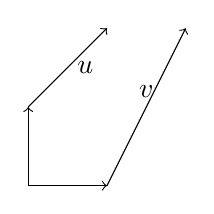
\begin{tikzpicture}
			\draw[->] (0,0) -- (1,0);
			\draw[->] (0,0) -- (0,1);
			\draw[->] (0,1) -- (1,2) node[midway,right]{$u$};
			\draw[->] (1,0) -- (2,2) node[midway,above]{$v$};
		\end{tikzpicture}
	\end{center}
	Now we can start solving diophantine equations for $u,v$, knowing that the determinant of the \red{outward} edge
	vectors is $\pm 1$. In particular, one sees that $u_1 = \pm 1$ and $v_2 = \pm 1$ and $u_1v_2 - u_2v_1 = \pm 1$.

	\hfill

	Now one makes some simplifications, and comes to the cases $u_2v_1 = 0$ or $u_2v_1 = 2$. The first case
	gives us another right angle and the resulting family of Hirzebruch surfaces $H_a$. In fact
	these are all of the toric symplectic manifolds with four fixed points. Perhaps an algebraic
	geometer would say that these are all of the $\C\P^1$ bundles over $\C\P^1$.
	\begin{center}
		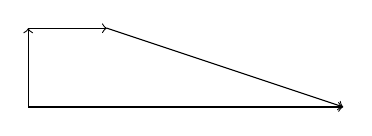
\begin{tikzpicture}
			\draw[->] (0,0) -- (0,1);
			\draw[->] (0,0) -- (4,0);
			\draw[->] (0,1) -- (1,1);
			\draw[->] (1,1) -- (4,0);
		\end{tikzpicture}

		This is the polytope for $H_3$ where $3$ indexes the slope of the line.
	\end{center}

	If we consider the other case, we actually end up in the following situation \begin{center}
		\begin{tikzpicture}
			\draw (0,0) -- (2,4);
			\draw (2,4) -- (2,3);
			\draw (2,3) -- (3,3);
			\draw (3,3) -- (0,0);
		\end{tikzpicture}
	\end{center}
	In particular this polygon \red{is not convex} and hence is not the
	image of the moment map of a toric symplectic manifold.
	The curious thing is that it is smooth and simple. \red{is there any reasonable way of making sense
		of this?}
\end{example}

\begin{example}
	Take a Delzant polytope in $\R^n$ with a vertex $p$ and with primitive inward pointing
	edge vectors $u_1,\dots,u_n$ at $p$. Chop off the corner to obtain a new polytope with the same
	vertices except $p$, and with $p$ replaced by the new vertices $p + \varepsilon u_1,\dots,p + \varepsilon u_n$.

    \hfill

    Show that the new polytope is Delzant.

    \hfill

    Smoothness is the only thing worth considering, and we only have to check at each of the new vertices.
    At the $j$ vertex, the inward pointing edge vectors are $u_j$ and $u_i - u_j$ for $i\neq j$. These clearly $\Z$-basis
    the lattice.
\end{example}

\begin{example}
    Show that the Hirzebruch surface $H_a$ is a symplectic reduction of $\C^4$ with respect to an action of $(S^1)^2$.
    Exhibit $H_a$ as a $\C\P^1$ bundle over $\C\P^1$. \red{I have no idea how to do this}
\end{example}

\begin{example}
    Which $2n$-dimensional toric manifolds have exactly $n+1$ fixed points?

    \hfill

    The answer is $\C\P^n$ with the standard action of $T^n$. What we are asking for is all Delzant polytopes 
    in $\R^n$ with $n+1$ vertices. The only such polytope is the standard simplex.

    \hfill

    To see this, use the $\SL_n(\Z)$ action to make one vertex a right angle. Then the rest of the vertices
    must lie on the standard basis vectors. Then we see that the rest of the edge vectors have exactly two nonzero 
    coordinates. At each vertex we are thinking about the following determinant \begin{align*}
        \begin{bmatrix}
            1 & 0 & 0 & 0 & 0 \\
            * & * & 0 & 0 & 0 \\
            * & 0 & * & 0 & 0 \\
            * & 0 & 0 & * & 0 \\
            * & 0 & 0 & 0 & *
        \end{bmatrix}
    \end{align*} and this has to equal $\pm 1$. 
\end{example}

\section{Projective GIT quotients}
The point of what I understand here is that there is a choice of something in symplectic/algebraic geometry stories.
In the symplectic story, the construction is up to choice of moment map, and in the algebraic story, the construction
is up to choice of linearization of the action. 

\hfill

\red{To understand!!}
\begin{remark}
    We define the quotient of $\Proj R$ by $G$ 
in terms of the ring $R$ but it is not possible to recover $R$ from $\Proj R$. Under suitable conditions,
$R$ is the ring of functions on the total space of the tautoological line bundle over $\Proj R$. Thus
in this case the projective GIT quotient is determined by the action of $G$ on the tautological line bundle.
A lift of a $G$-action from $X$ to $O_X(-1)$ is often called a linearization of the action.
\end{remark}
\subsection{The third construction}

\subsection{The fourth construction}

\section{References}
\begin{itemize}
	\item Proudfoot toric variety notes
	\item Allen Horn problem notes
	\item A review of Lie Group Actions and the Notion of Moment Map Daniel Rutschmann
	\item Ana Cannas da Silva, Lectures on Symplectic Geometry
	\item Lee Smooth
\end{itemize}
\end{document}